\chapter{(eXtended) Cellular Automata}

Cellular Automata (CA) are parallel computing models, whose evolution
is ruled by local rules. A cellular automaton can be thought as a
$d$-dimensional space, the \emph{cellular space}, subdivided in
regular cells of uniform shape and size. Each cell embeds a
\emph{finite automaton}, that is one of the most simple and well known
computational model in Computer Science and can assume a finite number
of states. At time $t=0$, cells are in arbitrary states and the CA
evolves step by step by changing the states of the cells at discrete
time steps, by applying the same local rule of evolution, i.e. the
cell's \emph{transition function}, simultaneously (i.e. in parallel)
to each cell of the CA. Input for the cell is given by the states of a
predefined set of neighboring cells, which is assumed constant in
space and time.

It is possible to indentify an informal definition of cellular
automaton by simply listing it main properties:

\begin{itemize}
\item It is formed by a $d$-dimensional space, called \emph{cellular
  space}, partitioned into cells of uniform shape (triangles, squared,
  hexagons, cubes) and size (see Figure \ref{fig:cellularspaces});
\item The number of cell states is finite;
\item The evolution occurs through discrete steps;
\item Each cell evolves by simultaneously changing its state by
  applying the same transition function to the cellular space;
\item The transition function depends on the state of the central and
  neighboring cells
\item The relationship of closeness that defines the neighborhood of a
  cell is local, uniform and invariant over time.
\end{itemize}

\begin{figure}
  \begin{center}
    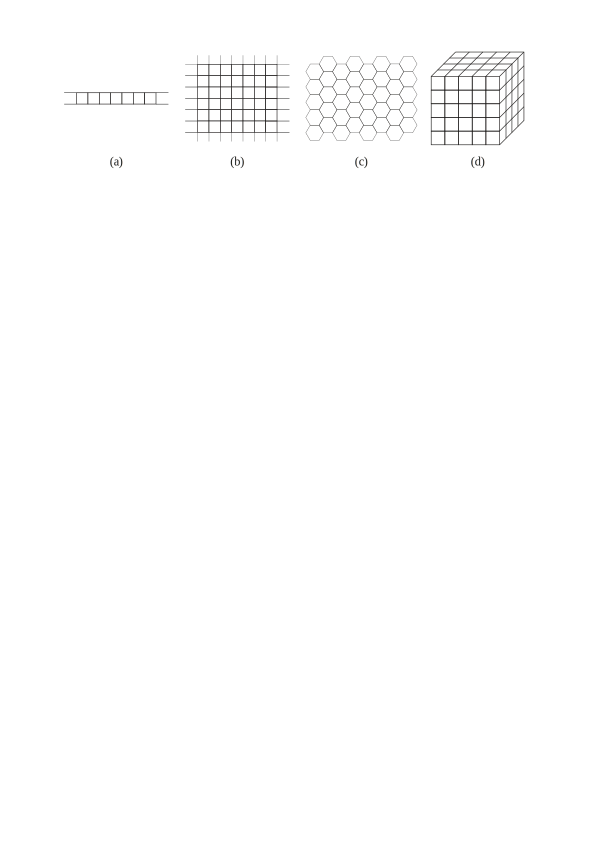
\includegraphics[width=12cm]{./images/CellularAutomata/cellularspaces}
    \caption{Example of cellular spaces: (a) one-dimensional, (b)
      two-dimensional with square cells, (c) two-dimensional with
      hexagonal cells, (d) three-dimensional with cubic cells.}
    \label{fig:cellularspaces}
  \end{center}
\end{figure}

The cell's relationship of closeness depends on the geometry. Figures
\ref{fig:1Dneighborhood} and \ref{fig:2Dneighborhood} show examples of
1D and 2D neighborhoods, respectively.

\begin{figure}
  \begin{center}
    \includegraphics[width=12cm]{./images/CellularAutomata/onedimensional.pdf}
    \caption{Example of neighborood with radius (a) $r
      = 1$ and (b) $r = 2$ for one-dimensional cellular automata.}
    \label{fig:1Dneighborhood}
  \end{center}
\end{figure}



\begin{figure}
  \begin{center}
    \includegraphics[width=12cm]{./images/CellularAutomata/twodimensional.pdf}
    \caption{von Neumann (a) and Moore (b) neighboroods for a
      two-dimensional cellular automata with square cells and with
      exagonal ones (c).}
    \label{fig:2Dneighborhood}
  \end{center}
\end{figure}


Despite their simple definition, CA can exhibit very interesting,
complex global behaviors. Moreover, from a computational point of
view, they are equivalent to Turing Machines. CA are particularly
adapt to model and simulate complex systems, i.e. those systems
characterized by interaction of numerous elementary constituents. As a
matter of fact, they have been largely employed different scientific fields.

\section{Formal Definition of Cellular Automata}

The homogeneous cellular automata is a quadruple:

$$A = <R,X,Q,\sigma>$$

\noindent where:

\begin{itemize}
\item $R = \{i = (i_1,i_2,....,i_d) \; | \; i_k \in \mathbb{Z} \;\; \forall k =
  1,2,...,d\}$ is the set of points, with integer coordinates, which
  defines the $d$-dimensional cellular space;

\item $X = \{\xi_0,\xi_1\,...\xi_{m-1}\}$ is the finite set of m
  $d$-dimensional vectors
  \[ \xi_j = \{\xi_{j1},\xi_{j2},...\xi_{jd}\} \]
  that define the set
  \[ N(X,i) = \{i + \xi_0,i + \xi_1,...,i + \xi_{m-1}\} \]
  of coordinates of cells close to the generic cell $i$ with
  coordintates $(i_1,i_2,...i_d)$. X is the geometrical pattern that
  specifies the neighbourhood relationship;
  
\item $Q$ is the finite set of states of the cellular automata;
  
\item $\sigma : Q^m \rightarrow Q$ is the transition function for the CA

\end{itemize}


\section{Some Applications of Cellular Automata}

CA are particularly suited to modeling and simulation of some classes
of complex systems characterized by the interaction of a large numebr
of elementary components. The assumption that if a system behaviour is
complex, the model that describes it must necessarily be of the same
complexitiy is replaced by the idea that its behavior can be
described, at least in some cases, in very simple terms.

Among different fields, fluid-dynamics is one of most important field
of application for CA and, in this research branch, many different
CA-based methods were used to simulate fluid flows. Lattice Gas
Automata models were introduced for describing the motion and
collision of “particles” on a grid and it was shown that such models
can simulate fluid dynamical properties. The continuum limit of these
models leads to the Navier-Stokes equations. Lattice Gas models can be
regarded as microscopic models, as they describe the motion of fluid
\emph{particles} which interact by scattering. An advantage of Lattice
Gas models is that the simplicity of particles, and of their
interactions, allow for the simulation of a large number of them,
making it therefore possible to observe the emergence of flow
patterns. Furthermore, since they are cellular automata systems, it
makes easily to run simulations with parallel computing. A different
approach to LGA is represented by Lattice Boltzmann models in which
the state variables can take continuous values, as they are supposed
to represent the density of fluid particles, endowed with certain
properties, located in each cell (here space and time are discrete, as
in lattice gas models). Both Lattice Gas and Lattice Boltzmann Models
have been applied for the description of fluid turbulence.

Because many complex natural phenomena evolve on very large areas,
they are therefore difficult to be modelled at a microscopic level of
description. Among these, we can find some real flow-type phenomena
like debris and lava flows, as well as flloods and pyroclastic
flows. Besides rehological complex behaviour, such flows generally
evolve on complex topographies that can change during the phenomenon
evolution per effcet of the flow itself, and are often characterised
by branching and rejoining of the flow. In order to better model such
kind of phenomena, an extended notion of Cellular Automata, described
in the next Section, can represent a valid alternative to classical
CA.

\section{eXtended Cellular Automata}

As regards the modeling of natural complex phenomena, Crisci and
co-workers proposed a method based on an eXtended notion of
homogeneous CA (XCA), firstly applied to the simulation of basaltic
lava flows \cite{Crisci1982}. XCA can greatly make more
straightforward the modeling of some complex systems, as those cited
in the previous Section. Note that the XCA method is also known as
Complex Cellular Automata, Macroscopic Cellular Automata
\cite{Spataro2010} or Multicomponent Cellular Automata
\cite{Avolio2012}.

Informally, XCA, compared to classical CA, are different because of
the following reasons:

\begin{itemize}

\item The state of the cell must account for all the characteristics,
  which are assumed to be relevant to the evolution of the system:
  these refer to the space portion of the cell. Each characteristic
  corresponds to a \emph{substate}. The state of the cell is divided
  into substates and permitted values for a substate must form a
  finite set. The set of the possible states of a cell represents the
  global state of the cell and is given by the Cartesian product of
  the sets of the substates.

\item As the state of the cell can be decomposed in substates, also
  the cell's transition function can be split into \emph{elementary
    processes}. Each of them represents a particular aspect that rules
  the dynamic of the considered phenomenon.

\item A set of \emph{parameters} to reproduce the several different
  dynamic behaviors of the considered phenomenon is defined.

\item Global operations can be allowed, (e.g. to model external
  influences that can not easily be described in terms of local
  interactions, or to perdorm reductions over the whole, or a subset of,
  the cellular space). Such operation go under the name of
  \emph{steering}.
  
\end{itemize}

\noindent Formally, a XCA is a 7-tuple:

$$ A = <R,X,Q,P,\sigma,E,\gamma>$$

\noindent where:

\begin{itemize}

\item $R$ is the $d$-dimensional cellular space;

\item $X$ is the geometrical pattern that specifies the neighbourhood relationship;

\item $Q = Q_1 \times Q_2 \times....\times Q_n$ is the set of states
  of the cell obtained as the Cartesian product of \emph{substates}
  $Q_1 \times Q_2 \times....\times Q_n$ each one representing a
  particular feature of the phenomenon to be modelled;

\item $P = {p_1,p_2,....,p_p}$ is the set of CA \emph{parameters}.They
  allow to “tune” the model for reproducing different dynamical
  behaviours of the phenomenon of interest;

\item $\sigma : Q^m \rightarrow Q$ is the transition function for the
  CA and it is splitted in \emph{elementary processes} $\tau_1,\tau_2,
  ..., \tau_s$, each one describing a particular aspect that rules the
  dynamic of the considered phenomenon.

\item $\gamma: \Gamma \rightarrow Q^{|\Gamma|} \times \mathbb{R}$ is
  the (global) steering functions. Here, $\Gamma \subseteq R$ is a
  subset of cells of the cellular space, while $\mathbb{R}$ the set of
  real numbers.

\end{itemize}


In the next Chapter, same examples of XCA will be presented and
implemented in OpenCAL.

